\newpage
%\addcontentsline{toc}{chapter}{\MakeUppercase{System Architecture}}
\thispagestyle{empty}
%
\begin{spacing}{1.2}
%
\chapter{System Architecture}

This chapter presents the architectural design of the GramaGIS system, detailing how its core components are structured and interconnected to deliver a secure, intelligent, and scalable Panchayat management platform. Each section traces the evolution of key subsystems from spatial data delivery and natural language querying to administrative data management, illustrating the engineering decisions that shaped the final implementation.

\section{Architecture Diagram}

\begin{figure}[H]
    \centering
    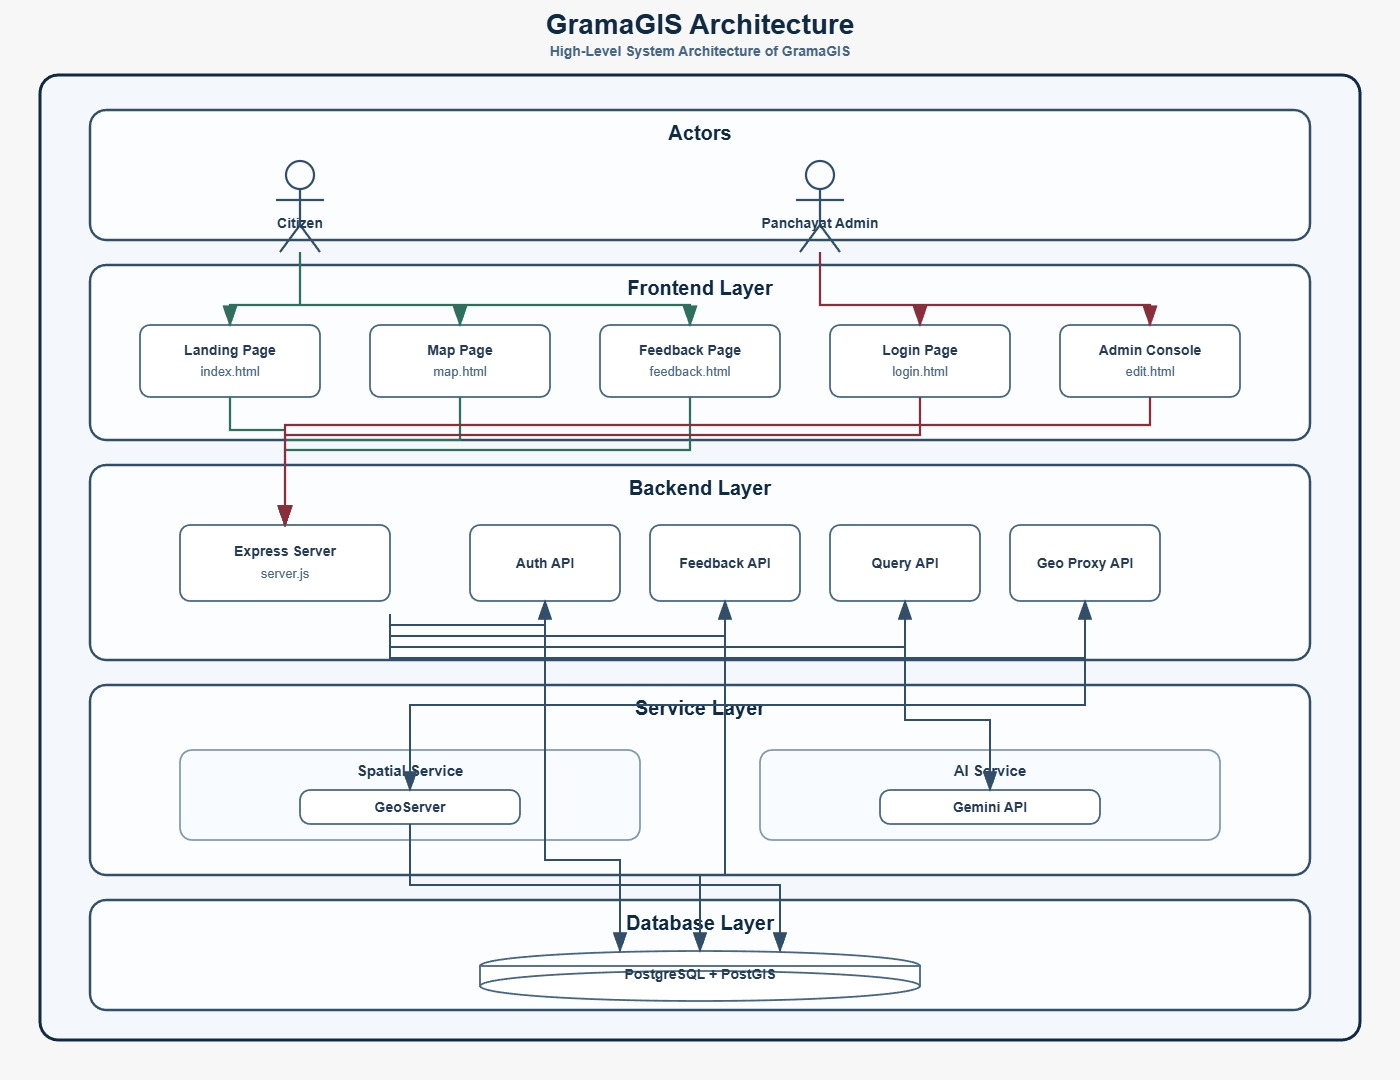
\includegraphics[width=1\linewidth]{Images/Arch.jpeg}
    \caption{Architectural Diagram}
    \label{fig:Architectural Diagram}
\end{figure}

\section{Architectural Design Evolution}

The structural design of GramaGIS was developed through a targeted evaluation of how to best serve rural administrative needs. Rather than adopting a generic GIS template, the architecture was engineered to solve three practical challenges: efficient map delivery, AI-assisted natural language querying, and protected administrative editing of spatial data. By iteratively testing different configurations, the final model evolved into a hybrid architecture in which public map rendering remains lightweight while authenticated workflows are routed through Express.js \cite{fu2020webgis}.

\section{Spatial Layer Management Architecture}

\subsection{Direct-to-GeoServer Architecture}

The initial implementation utilized a direct connection between the Leaflet frontend and GeoServer. Layers were requested using standard WMS/WFS calls directly to the GeoServer port (8080). While this allowed for rapid prototyping, it exposed the GeoServer URL and workspace details in the browser's network tab, leaving the core spatial engine vulnerable to unauthorized queries.

\subsection{Hybrid Express.js-Assisted Architecture}

To improve maintainability and secure administrative workflows, the implemented architecture adopts a hybrid \textbf{Express.js-assisted design}. The Express server acts as the application backend for authentication, feedback, natural language querying, protected WFS access, downloads, and transactional edits, while GeoServer continues to serve public WMS map layers directly to the browser.

The architectural flow is:
\begin{center}
PostgreSQL/PostGIS $\rightarrow$ GeoServer $\rightarrow$ Leaflet Frontend
\newline
and
\newline
Leaflet Frontend $\rightarrow$ Express.js API $\rightarrow$ Gemini / GeoServer / Database
\end{center}

In the implemented hybrid model, the frontend still communicates with GeoServer for direct WMS map rendering and feature inspection, but protected and structured workflows are routed through Express.js. This includes authentication, schema discovery, WFS querying for search results, dataset export, WFS-T-based edits, and feedback management. As a result, administrative credentials remain masked, edit operations can be authenticated, and AI-assisted queries can be validated before being applied to live data.

\section{NLP Intelligent Query Architecture}

The NLP subsystem is implemented as an Express.js route-driven module that coordinates translation from English queries to spatial filters.

\subsection{Intelligent NL2CQL Engine via Express}

The intelligence of GramaGIS lies in its ability to abstract complex spatial querying through an Express.js-managed NLP pipeline. Rather than allowing the LLM to generate raw SQL, the system utilizes the Gemini API to generate CQL (Command Query Language) filters \cite{liu2025nalspatial}. CQL is the native filtering language for GeoServer, allowing efficient live filtering without requiring direct SQL access from the browser.

The interaction follows a structured schema-aware workflow:

\begin{enumerate}
\item \textbf{Contextual Injection:} When a user enters a query (e.g., ``Find all schools in Ward 4''), the frontend sends the query and schema hint to the \textbf{Express.js backend}, which forwards the prompt to Gemini.
\item \textbf{NL2CQL Translation:} The AI processes the natural language and returns a structured JSON object containing the target layer and CQL filter.
\item \textbf{Filter Application:} The frontend applies the returned CQL filter to the relevant map layer and also requests filtered feature data through the Express WFS proxy.
\item \textbf{Dynamic Rendering:} GeoServer parses the CQL, fetches the specific rows from PostGIS \cite{postgis_in_action}, and returns filtered spatial results to the interface.
\end{enumerate}

\section{Administrative Data Management Architecture}

A foundational requirement was to move beyond a static map and provide a fully functional \textbf{Transactional GIS (T-GIS)}. This ensures that Panchayat officials can maintain a ``living'' database reflecting real-time changes in village infrastructure \cite{smart_panchayat2023}.

\subsection{Secure Transactional Proxy}

To allow for secure data modification, the architecture utilizes a \textbf{WFS-T (Web Feature Service-Transactional)} proxy within Express.js. This design ensures that the management module is robust enough for official use while remaining hidden from the public.

\subsection{The Data Management Process}

The process of managing data follows a multi-tier validation workflow:
\begin{enumerate}
    \item \textbf{Authentication:} The admin logs into the portal, the backend validates credentials against the login table, and a JSON Web Token (JWT) is issued for authenticated requests.
    \item \textbf{Client-Side Interaction:} The admin edits feature attributes through forms and, for editable geometries, uses the custom mini-map geometry editor to generate updated WKT values.
    \item \textbf{Backend Proxying:} The Express server validates the token and converts the update payload into a WFS-T XML transaction request using internal administrative credentials.
    \item \textbf{Database Commitment:} GeoServer executes the transaction on the PostGIS database, ensuring spatial integrity \cite{postgis_in_action}.
\end{enumerate}

\section{Summary of System Stack}

The final architecture unifies several specialized components into a single digital platform:
\begin{itemize}
    \item \textbf{PostgreSQL/PostGIS:} Database layer for spatial tables, feedback records, and login data \cite{postgis_in_action}.
    \item \textbf{GeoServer:} OGC-compliant map server for WMS, WFS, and WFS-T delivery \cite{fu2020webgis}.
    \item \textbf{Express.js:} Application backend for authentication, feedback, protected proxy routes, downloads, and NLP coordination.
    \item \textbf{Gemini API:} Natural language processing engine for query translation \cite{liu2025nalspatial}.
    \item \textbf{Leaflet.js:} Lightweight frontend library for interactive map visualization.
\end{itemize}

\end{spacing}
